\chapter{Application to hardcore point processes}

We want to apply our scale selection pipeline to a special kind of random point fields, namely hard-core models. A hard-core point field is characterized by the fact that two distinct points have a distance of at least $2R$ from each other. The parameter $R>0$ is called hardcore radius. In Section~\ref{sec:PPP} we quickly introduce the Poisson Point Process (PPP), since this process serves as starting point for most hardcore point processes. We will describe different kind of hardcore processes constructed from the PPP in Section~\ref{sec:hardcore_from_ppp}. Afterwards, we apply our scale selection pipeline to these processes in Section~\ref{sec:opt_scale_point_fields}.



\section{Poisson Point Process}\label{sec:PPP}

In this section, we give a brief but rigorous overview on Poisson point processes and hard-core models.

Define the set of locally finite subsets in $\mathbb{R}^d$ by
\begin{align*}
    \mathcal{C}:=\{\gamma\subseteq\mathbb{R}^d:\gamma_{\Lambda}:=\gamma\cap\Lambda\text{ is finite for any bounded set }\Lambda\subseteq\mathbb{R}^d\}
\end{align*}

Define the counting function $N_{\Lambda}$ on $\mathcal{C}$ by $N_{\Lambda}(\gamma):=\#\gamma_{\Lambda}$ for any bounded measurable set $\Lambda\subseteq\mathbb{R}^d$. We equip $\mathcal{C}$ with the $\sigma$-algebra $\mathcal{F}_{\mathcal{C}}$ which is generated by $N_{\Lambda}$, that is the smallest $\sigma$-algebra over $\mathcal{C}$ that contains the following family of sets:
\begin{align*}
    \{N_{\Lambda}^{-1}(A):A\subseteq\mathbb{N}_0,\Lambda\subseteq\mathbb{R}^d\text{ bounded measurable}\}
\end{align*}

A point process is a measurable function $\Gamma$ from a probability space $(\Omega,\mathcal{F},\mathbb{P})$ to $(\mathcal{C},\mathcal{F}_{\mathcal{C}})$. The distribution of $\Gamma$ is defined to be $\mathbb{P}(\Gamma\in F)$, $F\in\mathcal{F}_{\mathcal{C}}$.

Let $\mu$ be a $\sigma$-finite measure on $\mathbb{R}^d$. A Poisson point process with intensity $\mu$ is a point process $\Gamma$ such that for any bounded $\Lambda\subseteq\mathbb{R}^d$ we have
\begin{itemize}
    \item $N_{\Lambda}(\Gamma)\sim\text{Poi}(\mu(\Lambda))$
    \item Given the event $\{N_{\Lambda}(\Gamma)=n\}$, the $n$ points in $\Gamma_{\Lambda}$ are independent and distributed following the distribution $\mu_{\Lambda}/\mu(\Lambda)$. Here, $\mu_{\Lambda}$ is the restriction of $\mu$ on $\Lambda$: $\mu_{\Lambda}(A):=\mu(\Lambda\cap A)$. This means:
    \begin{align*}
        \mathbb{P}(X_1\in A_1,\dots,X_n\in A_n|N_{\Lambda}(\Gamma)=n)=\prod_{i=1}^{n}\frac{\mu_{\Lambda}(A_i)}{\mu(\Lambda)}
    \end{align*}
    for all measurable $A_i\subseteq\Lambda$, $i=1,\dots,n$
\end{itemize}

Often times, we just set $\mu=\xi\lambda^d$, where $\lambda^d$ is the $d$-dimensional Lebesgue measure and $\xi>0$ the intensity.

Notation:
\begin{itemize}
    \item $\pi^{\xi}$ distribution of Poisson point process with intensity $\mu=\xi\lambda^d$
    \item $\pi^{\xi}_{\Lambda}$ distribution of Poisson point process with intensity $\mu=\xi\lambda^d_{\Lambda}$ 
    \item $\mathcal{C}_f=\{\gamma\in\mathcal{C}:\gamma\text{ is finite}\}$
\end{itemize}

\section{Hardcore processes constructed from Poisson point processes}\label{sec:hardcore_from_ppp}

\subsection{Matern type 1 and 2 processes}

One way to generate Hard-core processes is to first generate a Poisson point process and then thin out point using a specified rule. 

Matern Type 1 process:

Matern Type 2 process:

\begin{figure}[ht]
    \centering
    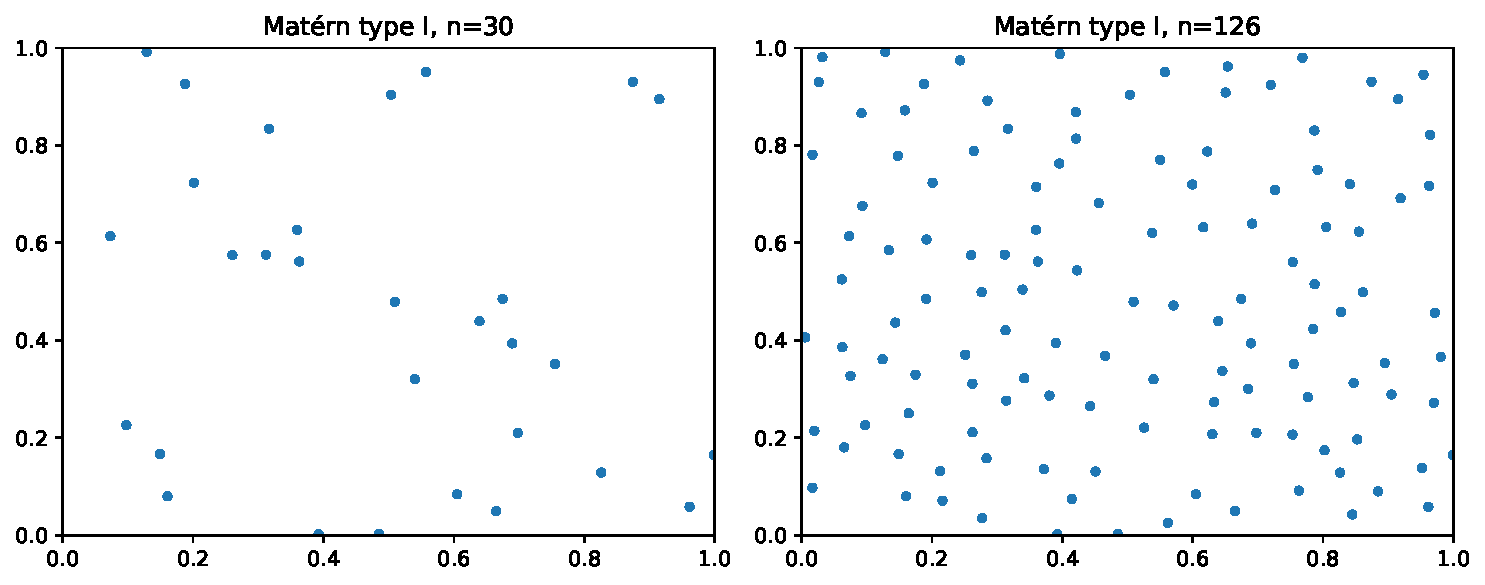
\includegraphics[width=\linewidth]{Abschlussarbeit_2021/LaTeX/images/matern_type_I_II.pdf}
    \caption{intensity of underlying Poisson point process: $\lambda_{P}=300$, hard-core radius: $R=0.025$}
    \label{fig:matern}
\end{figure}

\subsection{Gibbs process}

\begin{Def}[Gibbs-process]
    Let $z>0$ be the activity, $\beta\ge0$ inverse temperature and $H$ and energy function. Let $\Lambda\subseteq\mathbb{R}^d$ be bounded. The Gibbs measure on $\Lambda$ is the distribution given by
    \begin{align*}
        P_{\Lambda}^{z,\beta}=\frac{1}{Z_{\Lambda}^{z,\beta}}z^{N_{\Lambda}}e^{-\beta H}\pi_{\Lambda},
    \end{align*}
    where $Z_{\Lambda}^{z,\beta}$ is the normalization constant of $\int z^{N_{\Lambda}}e^{-\beta H}d\pi_{\Lambda}$
\end{Def}

Special case of Gibbs processes: Strauss process

\section{Optimal Scale for Point Fields}\label{sec:opt_scale_point_fields}

Let $S_n=\{x_1,\dots,n\}$ be a point cloud with $d(x,y)\ge R$ for all $x,y\in S$, $x\ne y$. Define $\rho_n=\min\{d(x,y):x,y\in S,x\ne y\}$. Then $\rho_n\ge R$. It is natural to consider settings in which $\rho_n\to R$ for $n\to\infty$. $S_n$ could be the realization of a hardcore point field.

\todo[inline]{Find some kind of result comparable to $\rho_n\to R$}

We would like to recover the hard-core radius $R$ using our scale selection pipeline. This serves only as a toy example, because a natural estimate for $R$ would be the minimum distance between two distinct points: $\hat{R}=\rho_n$.

We want to have a functional $f$ that peaks around the hardcore radius $R$. If we use $\beta_0$ we get a monotonously decreasing functional that starts to decrease around $\epsilon=\rho_n$. For $\epsilon<\rho_n$ the functional is constant and equal to the number of points in the point cloud. See Figure []. Of course we can restrict the functional $f=\beta_0$ to an interval $[\epsilon_{\min},\epsilon_{\max}]$ where it is (strictly) monotonously decreasing and then apply the scale selection procedure for monotone functionals from Section [].

We will also try $f=\beta_0-\beta_1$ and $f=\alpha\beta_0+\gamma\beta_1$. See Figure [].

\subsubsection*{Conjecture}

Consider a filtration $K_{\epsilon}(S_n)$ on the grid $0<\epsilon_1<\dots<\epsilon_N<\operatorname{diam}(S_n)/2$. Let the functional $f$ be given by $f_{\alpha}(K)=\beta_0(K)^{\alpha}\cdot f_1(K)^{\gamma}$ for some parameters $\alpha,\gamma>0$. Let $\Sigma_N$ be the resulting scale similarity matrix, $v^*$ the principal eigenvector and $\epsilon_{\text{crit}}=\epsilon_{j_{\text{crit}}}$, where $j_{\text{crit}}\in\arg\max\{v^*_j:j=1,\dots,N\}$. Note that the selected scale $\epsilon_{\text{crit}}$ depends on the parameters $\alpha$, $\gamma$, $N$ and $n$. It holds
\begin{align*}
    \lim\limits_{\alpha\to\infty,\gamma\to0}\epsilon_{\text{crit}}=\arg\min\limits_{j=1,\dots,N}\{\epsilon_j:|\epsilon_j-\rho_n|\}
\end{align*}
If we make the grid finer ($N\to\infty$), we would get
\begin{align*}
    \lim\limits_{N\to\infty}\lim\limits_{\alpha\to\infty}\epsilon_{\text{crit}}=\rho_n
\end{align*}
Finally if we sample more and more points ($n\to\infty$)
\begin{align*}
    \lim\limits_{n,N,\alpha\to\infty}\epsilon_{\text{crit}}=R
\end{align*}

